\documentclass[main.tex]{subfiles}
\begin{document}


\section{Rijen van Continue functies}
\label{sec:rijen-van-Continue-functies}

\begin{de}
  Beschouw een rij $(f_{n})_{n}$ van functies op een verzameling $A$ met waarden in $\mathbb{R}$ (of $\mathbb{C}$).
  We zeggen dat $(f_{n})_{n}$ \term{puntsgewijs convergeert} op $A$ naar een functie $f: A \rightarrow \mathbb{R}$ als het volgende geldt:
  \[ \forall x\in A:\ \epsilon \in \mathbb{R}_{0}^{+}:\ \exists n_{0}\in \mathbb{N}:\ \forall n\in \mathbb{N}:\ n \ge n \Rightarrow |f_{n}(x)-f(x)| < \epsilon \]
\end{de}

\begin{vb}
  De rij $(f_{n})_{n}$ convergeert puntsgewijs naar $f:\ \mathbb{R} \rightarrow \mathbb{R}:\ x \mapsto 0$.

  \noindent
  \begin{minipage}{.45\textwidth}
    \begin{figure}[H]
      \centering
      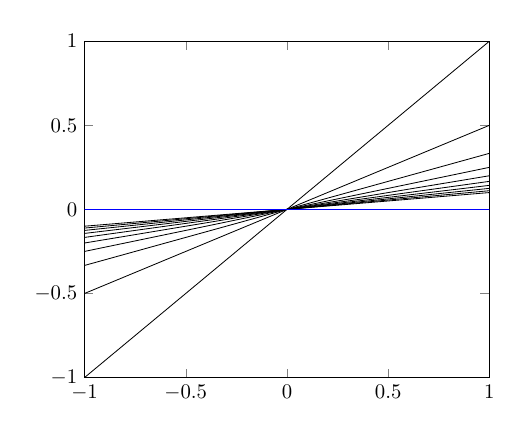
\begin{tikzpicture}[scale=.75]
        \begin{axis}[ymin=-1, ymax=1, xmin=-1, xmax=1]
          \foreach \i in {1,...,10}
          {\addplot[smooth,domain=-5:5]{x/\i};}
          \addplot[domain=-5:5,color=blue,thick]{0};
        \end{axis}
      \end{tikzpicture}
    \end{figure}
  \end{minipage}
  \begin{minipage}{.45\textwidth}
    \[ f_{n}:\ \mathbb{R} \rightarrow \mathbb{R}:\ x \mapsto \frac{x}{n} \]
  \end{minipage}
  \extra{bewijs}
\end{vb}

\begin{vb}
  de rij $(f_{n})_{n}$ convergeert puntsgewijs naar $f:\ \mathbb{R} \rightarrow \mathbb{R}:\ x \mapsto 1$.

  \noindent
  \begin{minipage}{.45\textwidth}
    \begin{figure}[H]
      \centering
      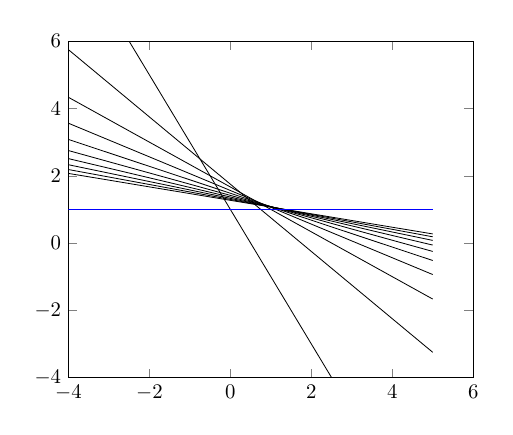
\begin{tikzpicture}[scale=.75]
        \begin{axis}[ymin=-4, ymax=6, xmin=-4, xmax=6]
          \foreach \i in {1,...,10}
          {\addplot[smooth,domain=-5:5]{1- (3/\i)*(x-1+(1/\i)) + (x/\i)};}
          \addplot[domain=-5:5,color=blue,thick]{1};
        \end{axis}
      \end{tikzpicture}
    \end{figure}
  \end{minipage}
  \begin{minipage}{.45\textwidth}
  \[ f_{n}:\ \mathbb{R} \rightarrow \mathbb{R}:\ x \mapsto 1- \frac{3}{n}\left(x-1+\frac{1}{n}\right) + \frac{x}{n} \]
  \end{minipage}
\extra{bewijs}
\end{vb}

\begin{vb}
  De rij $(f_{n})_{n}$ convergeert puntsgewijs naar $f:\ \mathbb{R} \rightarrow \mathbb{R}:\ x \mapsto \sin(x)$.
  \[ f_{n}:\ \mathbb{R} \rightarrow \mathbb{R}:\ x \mapsto \sin\left(\left(1+\frac{1}{n}\right)x\right) \]
  \noindent
  \begin{minipage}{.45\textwidth}
    \begin{figure}[H]
      \centering
      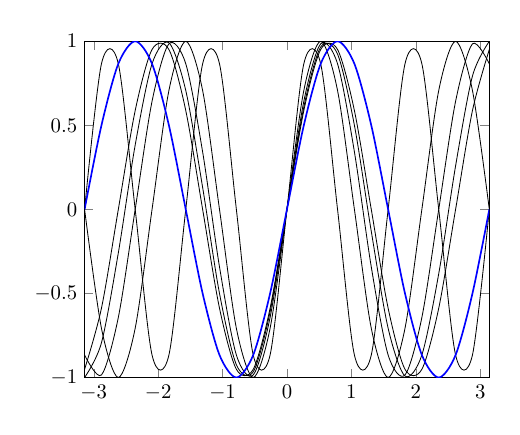
\begin{tikzpicture}[scale=.75]
        \begin{axis}[ymin=-1, ymax=1, xmin=-pi, xmax=pi]
          \foreach \i in {1,...,5}
          {\addplot[smooth,domain=-pi:pi]{sin((1+(1/\i))*x*(360/pi))};}
          \addplot[smooth,domain=-pi:pi,color=blue,thick]{sin(x*(360/pi))};
        \end{axis}
      \end{tikzpicture}
    \end{figure}
  \end{minipage}
  \begin{minipage}{.45\textwidth}
  \[ f_{n}:\ \mathbb{R} \rightarrow \mathbb{R}:\ x \mapsto \sin\left(\left(1+\frac{1}{n}\right)x\right) \]
  \end{minipage}
\extra{bewijs zodra de sinusfunctie gedefinieerd is.}
\end{vb}

\begin{vb}
  De rij $(f_{n})_{n}$ convergeert puntsgewijs naar $f$:

  \noindent
  \begin{minipage}{.45\textwidth}
    \begin{figure}[H]
      \centering
      \begin{tikzpicture}[scale=.75]
        \begin{axis}[ymin=-1.1, ymax=1.1, xmin=-1.1, xmax=1.1]
          \foreach \i in {1,...,10}
          {
            \addplot[smooth,domain=-3:(-1/\i)]{-1};
            \addplot[smooth,domain=(-1/\i):(1/\i)]{\i*x};
            \addplot[smooth,domain=(1/\i):3]{1};
          }
          \addplot[smooth,color=blue,thick,domain=-3:0]{-1};
          \addplot[smooth,color=blue,thick,domain=0:3]{1};
          \addplot[soldot,color=blue] coordinates{(0,0)};
          \addplot[holdot,color=blue,fill=white] coordinates{(0,1)(0,-1)};
        \end{axis}
      \end{tikzpicture}
    \end{figure}
  \end{minipage}
  \begin{minipage}{.45\textwidth}
  \[
  f_{n}: \mathbb{R} \rightarrow \mathbb{R}:\ x \mapsto
  \left\{
    \begin{array}{rl}
      -1 & \text{ als } x \in \interval[open left ]{-\infty}{-\frac{1}{n}}\\
      nx & \text{ als } x \in \interval[open      ]{-\frac{1}{n}}{\frac{1}{n}}\\
      1  & \text{ als } x \in \interval[open right]{\frac{1}{n}}{+\infty}\\
    \end{array}
  \right.
  \]
  \[
  f: \mathbb{R} \rightarrow \mathbb{R}:\ x \mapsto
  \left\{
    \begin{array}{rl}
      -1 & \text{ als } x \in \interval[open]{-\infty}{0}\\
      0  & \text{ als } x = 0\\
      1  & \text{ als } x \in \interval[open]{0}{+\infty}\\
    \end{array}
  \right.
  \]
  \end{minipage}
\extra{bewijs}
\end{vb}

\begin{vb}
  De rij $(f_{n})_{n}$ convergeert puntsgewijs naar $f$:

  \noindent
  \begin{minipage}{.45\textwidth}
    \begin{figure}[H]
      \centering
      \begin{tikzpicture}[scale=.75]
        \begin{axis}[ymin=-0.1, ymax=1.1, xmin=-3, xmax=3]
          \foreach \i in {1,...,10}
          {
            \addplot[smooth,domain=-3:3]{(\i^2*x^2)/(1+\i^2*x^2)};
          }
          \addplot[smooth,domain=-3:0,color=blue,thick]{1};
          \addplot[smooth,domain=0:3,color=blue,thick]{1};
          \addplot[soldot,color=blue] coordinates{(0,0)};
          \addplot[holdot,color=blue,fill=white] coordinates{(0,1)};
        \end{axis}
      \end{tikzpicture}
    \end{figure}
  \end{minipage}
  \begin{minipage}{.45\textwidth}
    \[
    f_{n}: \mathbb{R} \rightarrow \mathbb{R}:\ x \mapsto \frac{n^{2}x^{2}}{1 + n^{2}x^{2}}
    \]
    \[
    f: \mathbb{R} \rightarrow \mathbb{R}:\ x \mapsto
    \left\{
      \begin{array}{rl}
        0  & \text{ als } x = 0\\
        1  & \text{ als } x \neq 0\\
      \end{array}
    \right.
    \]
  \end{minipage}
  \extra{bewijs}
\end{vb}

\begin{vb}
  De rij $(f_{n})_{n}$ convergeert puntsgewijs naar $f$:

  \noindent
  \begin{minipage}{.45\textwidth}
    \begin{figure}[H]
      \centering
      \begin{tikzpicture}[scale=.75]
        \begin{axis}[ymin=-1.1, ymax=1.1, xmin=-0.1, xmax=1.1]
          \foreach \i in {1,...,10}
          {
            \addplot[smooth,domain=0:(1/(2*\i))]{2*\i*x};
            \addplot[smooth,domain=(1/(2*\i)):(1/\i)]{2-2*\i*x};
            \addplot[smooth,domain=(1/(\i)):1.1]{0};
          }
          \addplot[smooth,color=blue,thick,domain=-3:3]{0};
          \addplot[soldot,color=blue] coordinates{(0,0)};
        \end{axis}
      \end{tikzpicture}
    \end{figure}
  \end{minipage}
  \begin{minipage}{.45\textwidth}
  \[
  f_{n}: \mathbb{R} \rightarrow \mathbb{R}:\ x \mapsto
  \left\{
    \begin{array}{rl}
      2nx   & \text{ als } x \in \interval[open right]{0}{\frac{1}{2n}}\\
      2-2nx & \text{ als } x \in \interval{\frac{1}{2n}}{\frac{1}{n}}\\
      0     & \text{ als } x \in \interval[open left ]{\frac{1}{n}}{1}\\
    \end{array}
  \right.
  \]
  \[ f: \mathbb{R} \rightarrow \mathbb{R}:\ x \mapsto 0 \]
  \end{minipage}
\extra{bewijs}
\end{vb}

\begin{vb}
  De rij $(f_{n})_{n}$ convergeert puntsgewijs naar $f$:

  \noindent
  \begin{minipage}{.45\textwidth}
    \begin{figure}[H]
      \centering
      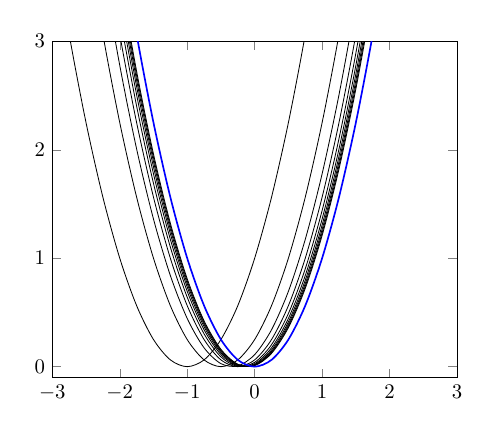
\begin{tikzpicture}[scale=.75]
        \begin{axis}[ymin=-0.1, ymax=3, xmin=-3, xmax=3]
          \foreach \i in {1,...,10}
          {
            \addplot[smooth,domain=-3:3]{(x+(1/\i))^2};
          }
          \addplot[smooth,color=blue,thick,domain=-3:3]{x^2};
        \end{axis}
      \end{tikzpicture}
    \end{figure}
  \end{minipage}
  \begin{minipage}{.45\textwidth}
  \[
  f_{n}: \mathbb{R} \rightarrow \mathbb{R}:\ x \mapsto \left(x+\frac{1}{n}\right)^{2}
  \]
  \[ f: \mathbb{R} \rightarrow \mathbb{R}:\ x \mapsto x^{2} \]
  \end{minipage}
\extra{bewijs}
\extra{convergeert ook uniform?}
\end{vb}

\begin{vb}
  De rij $(f_{n})_{n}$ convergeert puntsgewijs naar $f$:

  \noindent
  \begin{minipage}{.45\textwidth}
    \begin{figure}[H]
      \centering
      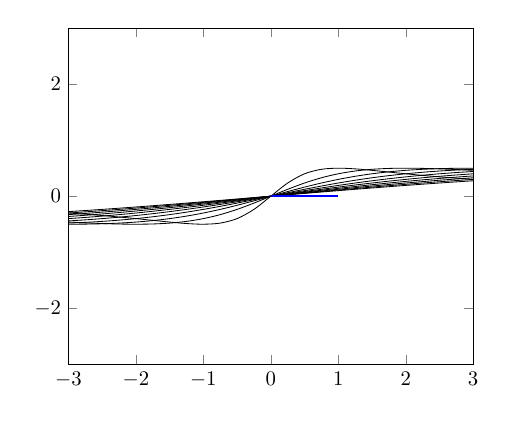
\begin{tikzpicture}[scale=.75]
        \begin{axis}[ymin=-3, ymax=3, xmin=-3, xmax=3]
          \foreach \i in {1,...,10}
          {
            \addplot[smooth,domain=-3:3]{(\i*x)/(\i^2+x^2)};
          }
          \addplot[smooth,color=blue,thick,domain=0:1]{0};
        \end{axis}
      \end{tikzpicture}
    \end{figure}
  \end{minipage}
  \begin{minipage}{.45\textwidth}
  \[
  f_{n}:\ \mathbb{R} \rightarrow \mathbb{R}:\ x \mapsto \frac{nx}{n^{2}+x^{2}}
  \]
  \[ f:\ \mathbb{R} \rightarrow \mathbb{R}:\ x \mapsto 0 \]
  \end{minipage}
\extra{bewijs}
\extra{convergeert ook uniform?}
\end{vb}

\begin{vb}
  De rij $(f_{n})_{n}$ convergeert puntsgewijs naar $f$:

  \noindent
  \begin{minipage}{.45\textwidth}
    \begin{figure}[H]
      \centering
      \begin{tikzpicture}[scale=.75]
        \begin{axis}[ymin=-0.1, ymax=1.1, xmin=-0.1, xmax=1.1]
          \foreach \i in {1,...,10}
          {
            \addplot[smooth,domain=0:1]{x^\i};
          }
          \addplot[smooth,color=blue,thick,domain=0:1]{0};
          \addplot[soldot,color=blue] coordinates{(0,0)};
          \addplot[holdot,color=blue,fill=white] coordinates{(1,0)};
        \end{axis}
      \end{tikzpicture}
    \end{figure}
  \end{minipage}
  \begin{minipage}{.45\textwidth}
  \[ f_{n}:\ \interval[open right]{0}{1} \rightarrow \mathbb{R}:\ x \mapsto x^{n} \]
  \[ f:\ \interval[open right]{0}{1} \rightarrow \mathbb{R}:\ x \mapsto 0  \]
  \end{minipage}
\extra{bewijs}
\extra{convergeert ook uniform?}
\end{vb}

\begin{vb}
  De rij $(f_{n})_{n}$ convergeert puntsgewijs naar $f$:

  \noindent
  \begin{minipage}{.45\textwidth}
    \begin{figure}[H]
      \centering
      \begin{tikzpicture}[scale=.75]
        \begin{axis}[ymin=-1.1, ymax=1.1, xmin=-3, xmax=3]
          \foreach \i in {1,...,10}
          {
            \addplot[smooth,domain=-3:3]{(x*\i)/(sqrt(1+(x*\i)^2))};
          }
          \addplot[smooth,color=blue,thick,domain=-3:0]{-1};
          \addplot[smooth,color=blue,thick,domain=0:3]{1};
          \addplot[soldot,color=blue] coordinates{(0,0)};
          \addplot[holdot,color=blue,fill=white] coordinates{(0,1)(0,-1)};
        \end{axis}
      \end{tikzpicture}
    \end{figure}
  \end{minipage}
  \begin{minipage}{.45\textwidth}
  \[
  f_{n}:\ \mathbb{R} \rightarrow \mathbb{R}:\ x \mapsto \frac{nx}{\sqrt{1+(nx)^{2}}}
  \]
  \[
  f: \mathbb{R} \rightarrow \mathbb{R}:\ x \mapsto
  \left\{
    \begin{array}{rl}
      -1 & \text{ als } x \in \interval[open]{-\infty}{0}\\
      0  & \text{ als } x = 0\\
      1  & \text{ als } x \in \interval[open]{0}{+\infty}\\
    \end{array}
  \right.
  \]
  \end{minipage}
\extra{bewijs}
\extra{convergeert ook uniform?}
\end{vb}

\begin{de}
  Beschouw een rij $(f_{n})_{n}$ van functies op een verzameling $A$ met waarden in $\mathbb{R}$ (of $\mathbb{C}$).
  We zeggen dat $(f_{n})_{n}$ \term{uniform convergeert} of \term{gelijkmatig convergeert} naar een functie $f: A \rightarrow \mathbb{R}$ als het volgende geldt:
  \[ \forall \epsilon \in \mathbb{R}_{0}^{+}:\ \exists n_{0} \in \mathbb{N}:\ \forall x \in A:\ \forall n\in \mathbb{N}:\ n \ge n_{0} \Rightarrow |f_{n}(x)-f(x)| < \epsilon \]
\end{de}

\begin{vb}
  Zij $f:\ A \rightarrow \mathbb{R}$ een willekeurige functie en $g:\ A \rightarrow \mathbb{R}$ een begrensde functie, dan convergeert de rij $(f_{n})_{n}$ uniforum op $A$ naar $f$:
  \[ f_{n}:\ f + \frac{1}{n}g \]

  \begin{proof}
    Kies een willekeurige $\epsilon \in \mathbb{R}_{0}^{+}$.
    Omdat $g$ begrensd is, bestaat er een $M \in \mathbb{R}^{+}$ als volgt:
    \[ \forall x \in A:\ |g(x)| \le M \]
    Kies $n_{0}\in \mathbb{N}$ nu zodat $n_{0} > \frac{M}{\epsilon}$ geldt.\lemref{lem:lemma-van-archimedes}
    Kies vervolgens een willekeurige $x\in A$ en $n \ge n_{0}$, dan geldt het volgende en volgt daaruit de uniforme convergentie:
    \[ |f_{n}(x) - f(x)| = \frac{1}{n}|g(x)| \le \frac{1}{n_{0}}M < \frac{\epsilon}{M}M = \epsilon \]
  \end{proof}
\end{vb}

\begin{vb}
  Beschouw de rij functies $(f_{n})_{n}$ als volgt:
  $(f_{n})_{n}$ convergeert puntsgewijs naar de nulfunctie maar niet uniform.

  \noindent
  \begin{minipage}{.45\textwidth}
    \begin{figure}[H]
      \centering
      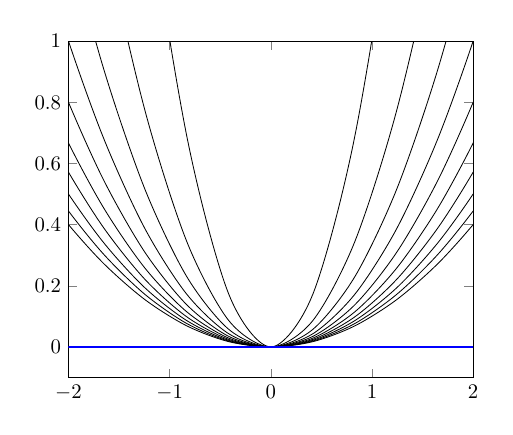
\begin{tikzpicture}[scale=.75]
        \begin{axis}[ymin=-0.1, ymax=1, xmin=-2, xmax=2]
          \foreach \i in {1,...,10}
          {\addplot[smooth,domain=-5:5]{x^2/\i};}
          \addplot[domain=-5:5,color=blue,thick]{0};
        \end{axis}
      \end{tikzpicture}
    \end{figure}
  \end{minipage}
  \begin{minipage}{.45\textwidth}
    \[ f_{n}:\ \mathbb{R} \rightarrow \mathbb{R}:\ x \mapsto \frac{1}{n}x^{2} \]
    \[ f:\ \mathbb{R} \rightarrow \mathbb{R}:\ x \mapsto 0 \]
  \end{minipage}
  \extra{bewijs puntsgewijze convergentie}

  \begin{proof}
    Kies $\epsilon = 1$ en een willekeurige $n_{0} \in \mathbb{N}$.
    Kies een $x \ge \sqrt{n_{0}}$ en $n = n_{0}$, dan geldt het volgende:
    \[ \frac{1}{n}x^{2} \ge \frac{1}{n_{0}}\left(\sqrt{n_{0}}\right)^{2} = 1 \ge \epsilon \]
  \end{proof}
\end{vb}

\begin{st}
  \label{str:uniform-dan-puntsgewijs}
  Een rij functies $(f_{n})_{n}$ die uniform convergeert, convergeert puntsgewijs.
\extra{bewijs}
\end{st}

\begin{tvb}
  Een rij functies $(f_{n})_{n}$ die puntsgewijs convergeert, convergeert niet noodzakelijk uniform.
\extra{tegenvoorbeeld}
\end{tvb}

\begin{bst}
  Beschouw een rij $(f_{n})_{n}$ van functies $f_{n}: A \subseteq \mathbb{R} \rightarrow \mathbb{R}$ die op $A$ uniform convergeert naar een functie $f:\ A \rightarrow \mathbb{R}$.
  \begin{itemize}
  \item Als $f_{n}$ continu is in een $a\in A$ voor elke $n$, dan is ook $f$ continu in $a$.
  \item Als $f_{n}$ uniform continu is op $A$ voor elke $n$, dan is ook $f$ uniform continu op $A$. 
  \end{itemize}

  \begin{proof}
    Rechtstreeks vanuit de definitie.
    \begin{itemize}
    \item 
      Kies een willekeurige $\epsilon \in \mathbb{R}_{0}^{+}$.
      Omdat $(f_{n})_{n}$ uniform convergeert naar $f$, kunnen we een $n_{0}\in \mathbb{N}$ vinden zodat voor alle $y\in A$ en voor alle volgende $n\in \mathbb{N}$ het volgende geldt:
      \[ |f_{n}(y)-f(y)|<\frac{\epsilon}{3} \]
      Omdat $f_{n}$ continu is in $a$ kunnen we een $\delta$ vinden
      zodat voor alle $x\in A$ uit $|x-a|<\delta$ het volgende geldt:
      \[ |f_{n}(x) - f_{n}(a) < \frac{\epsilon}{3} \]
      Voor elke $x\in A$ met $|x-a|<\delta$ geldt nu het volgende:
      \[
      \begin{array}{rl}
        |f(x)-f(a)| &= |f(x) - f_{n}(x) + f_{n}(x) - f_{n}(a) + f_{n}(a) - f(a)|\\
                    &\le |f(x) - f_{n}(x)| + |f_{n}(x) - f_{n}(a)| + |f_{n}(a) - f(a)|\\
                    &< \frac{\epsilon}{3} + \frac{\epsilon}{3} + \frac{\epsilon}{3}\\
                    &= \epsilon
      \end{array}
      \]
      $f$ is dus continu in $a$.
\extra{hermaken}
    \item
      Kies een willekeurige $\epsilon \in \mathbb{R}_{0}^{+}$.
      \begin{itemize}
      \item Omdat $(f_{n})_{n}$ uniform convergeert naar $f$ kunnen we een $n_{0} \in \mathbb{N}$ vinden zodat het volgende geldt voor alle $x \in A$ en alle $m \ge n_{0}$:
        \[ \forall x\in A, \forall m\ \in \mathbb{N}: m \ge n_{0} \Rightarrow |f(x)-f_{m}(x)| < \frac{\epsilon}{3} \]
      \item 
        Omdat $f_{n}$ uniforum continu is op $A$, kunnen we een $\delta \in \mathbb{R}_{0}^{+}$ vinden als volgt:
        \[ \forall x,y \in A:\  |x-y| < \delta \Rightarrow |f(x)-f(y)| < \frac{\epsilon}{3} \]
      \end{itemize}
      Voor elke $x,y \in A$ met $|x-y| < \delta$ vinden we nu het volgende:
      \[
      \begin{array}{rl}
        |f(x)-f(y)| &= |f(x)-f_{n}(x) + f_{n}(x) - f_{n}(y) + f_{n}(y) - f(y)|\\
                    &\le |f(x)-f_{n}(x)| + |f_{n}(x) - f_{n}(y)| + |f_{n}(ay) - f(y)|\\
                    &< \frac{\epsilon}{3} + \frac{\epsilon}{3} + \frac{\epsilon}{3}\\
                    &= \epsilon
      \end{array}
      \]
      $f_{n}$ is dus uniforum continu op $A$.
    \end{itemize}
  \end{proof}
\end{bst}



\end{document}
